Einmal im Jahr gibt es eine Woche in der alle Nationalparks keinen Eintritt kosten.
Dafür wird nach einer \FOREIGN{Donation}\footnote{Spende} gefragt.
Wir haben den letzten Tag dieser erwischt, entsprechend belebt war es.
Aber sicherlich nicht so belebt, wie in der Hochsaison.

\newpage
\thispagestyle{empty}
\begin{tikzpicture}[remember picture, overlay]
\node[inner sep=0pt, xshift=-.25\paperwidth, yshift=-.25\paperheight] (firerecovery) at (current page.north) {%
	\includegraphics[width=.5\paperwidth,height=.5\paperheight]{24/image20160424_090316880.jpg};%
};
\node[inner sep=0pt, text width=.35\paperwidth, align=justify, xshift=.2\paperwidth] at (firerecovery.east) {%
Vom Yosemite National Park Schild bis zum Passierhäuschen waren es wieder gute 30~Meilen.
Auf dem Weg dahin hielten wir an einem Aussichtspunkt an, von dem man das Resultat eines Waldbrandes betrachten konnte. Dort gab es eine Haltevorrichtung zum Fotografieren mit der Bitte das Foto auf einer \FOREIGN{social media} Plattform mit dem Lattenzaun \#rimfire01 zu posten.

Cleveres Outsourcen!
};
\end{tikzpicture}

\begin{tikzpicture}[remember picture, overlay]
\node[inner sep=0pt, yshift=.25\paperheight] at (current page.south) {%
	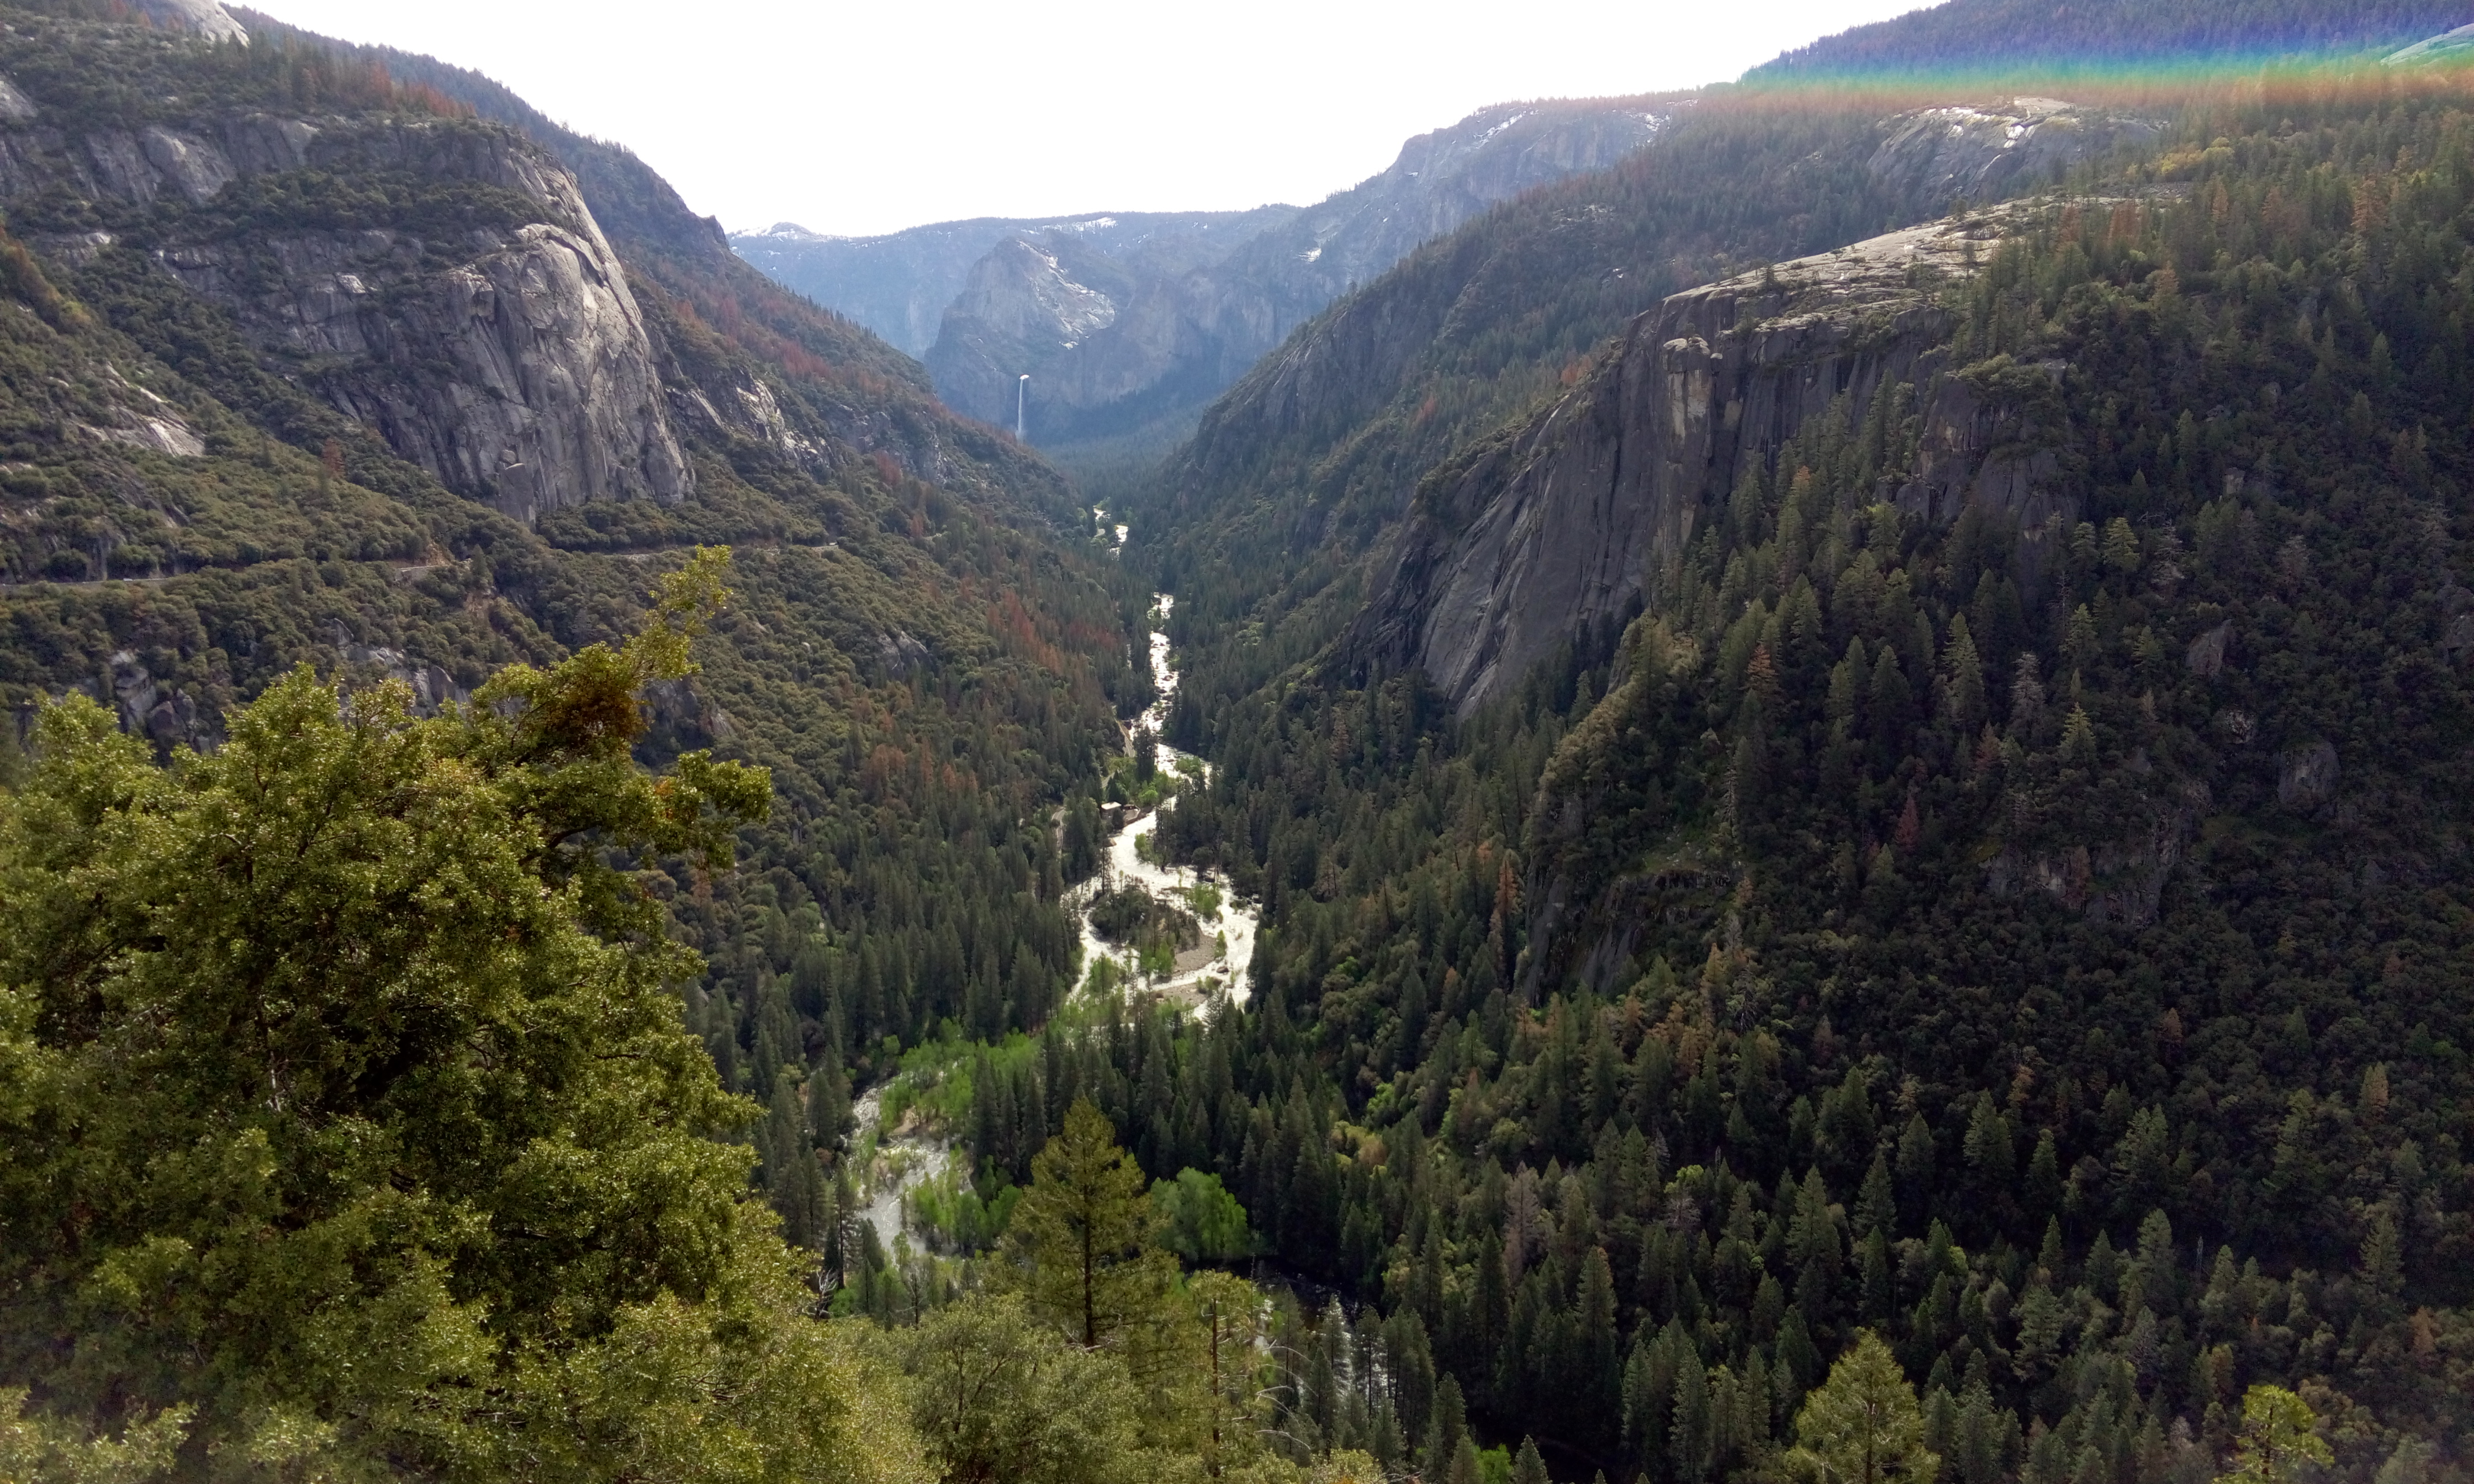
\includegraphics[angle=0,width=\paperwidth,height=.5\paperheight]{24/image20160424_095249873.jpg};%
};
\end{tikzpicture}

\newpage
\thispagestyle{empty}
\begin{tikzpicture}[remember picture, overlay]
\node[inner sep=0pt] at (current page.center) {%
	\includegraphics[width=\paperwidth,height=\paperheight]{24/image20160424_112102600.jpg};%
};
\end{tikzpicture}
\newpage

Wir sind ins Valley gefahren, um von dort den \FOREIGN{Upper Falls Trail} in Angriff zu nehmen.
Ich bin mit Winterjacke los und nach ein paar Höhenmeter in der Sonne habe ich mich darüber geärgert die Jacke überhaupt mitgenommen zu haben.
Der Trail war mit 5 bis 7 Stunden angegeben.
Nach rund 2~Stunden waren wir oben.
Dann schlug aber das Wetter um und was habe ich mich über meine Jacke gefreut.
Vollkommen durchnässt kamen wir dann am Auto an und fuhren nach Mariposa unserer Unterkunft.

\begin{tikzpicture}[remember picture, overlay]
\node[inner sep=0pt, yshift=.25\paperheight] at (current page.south) {%
	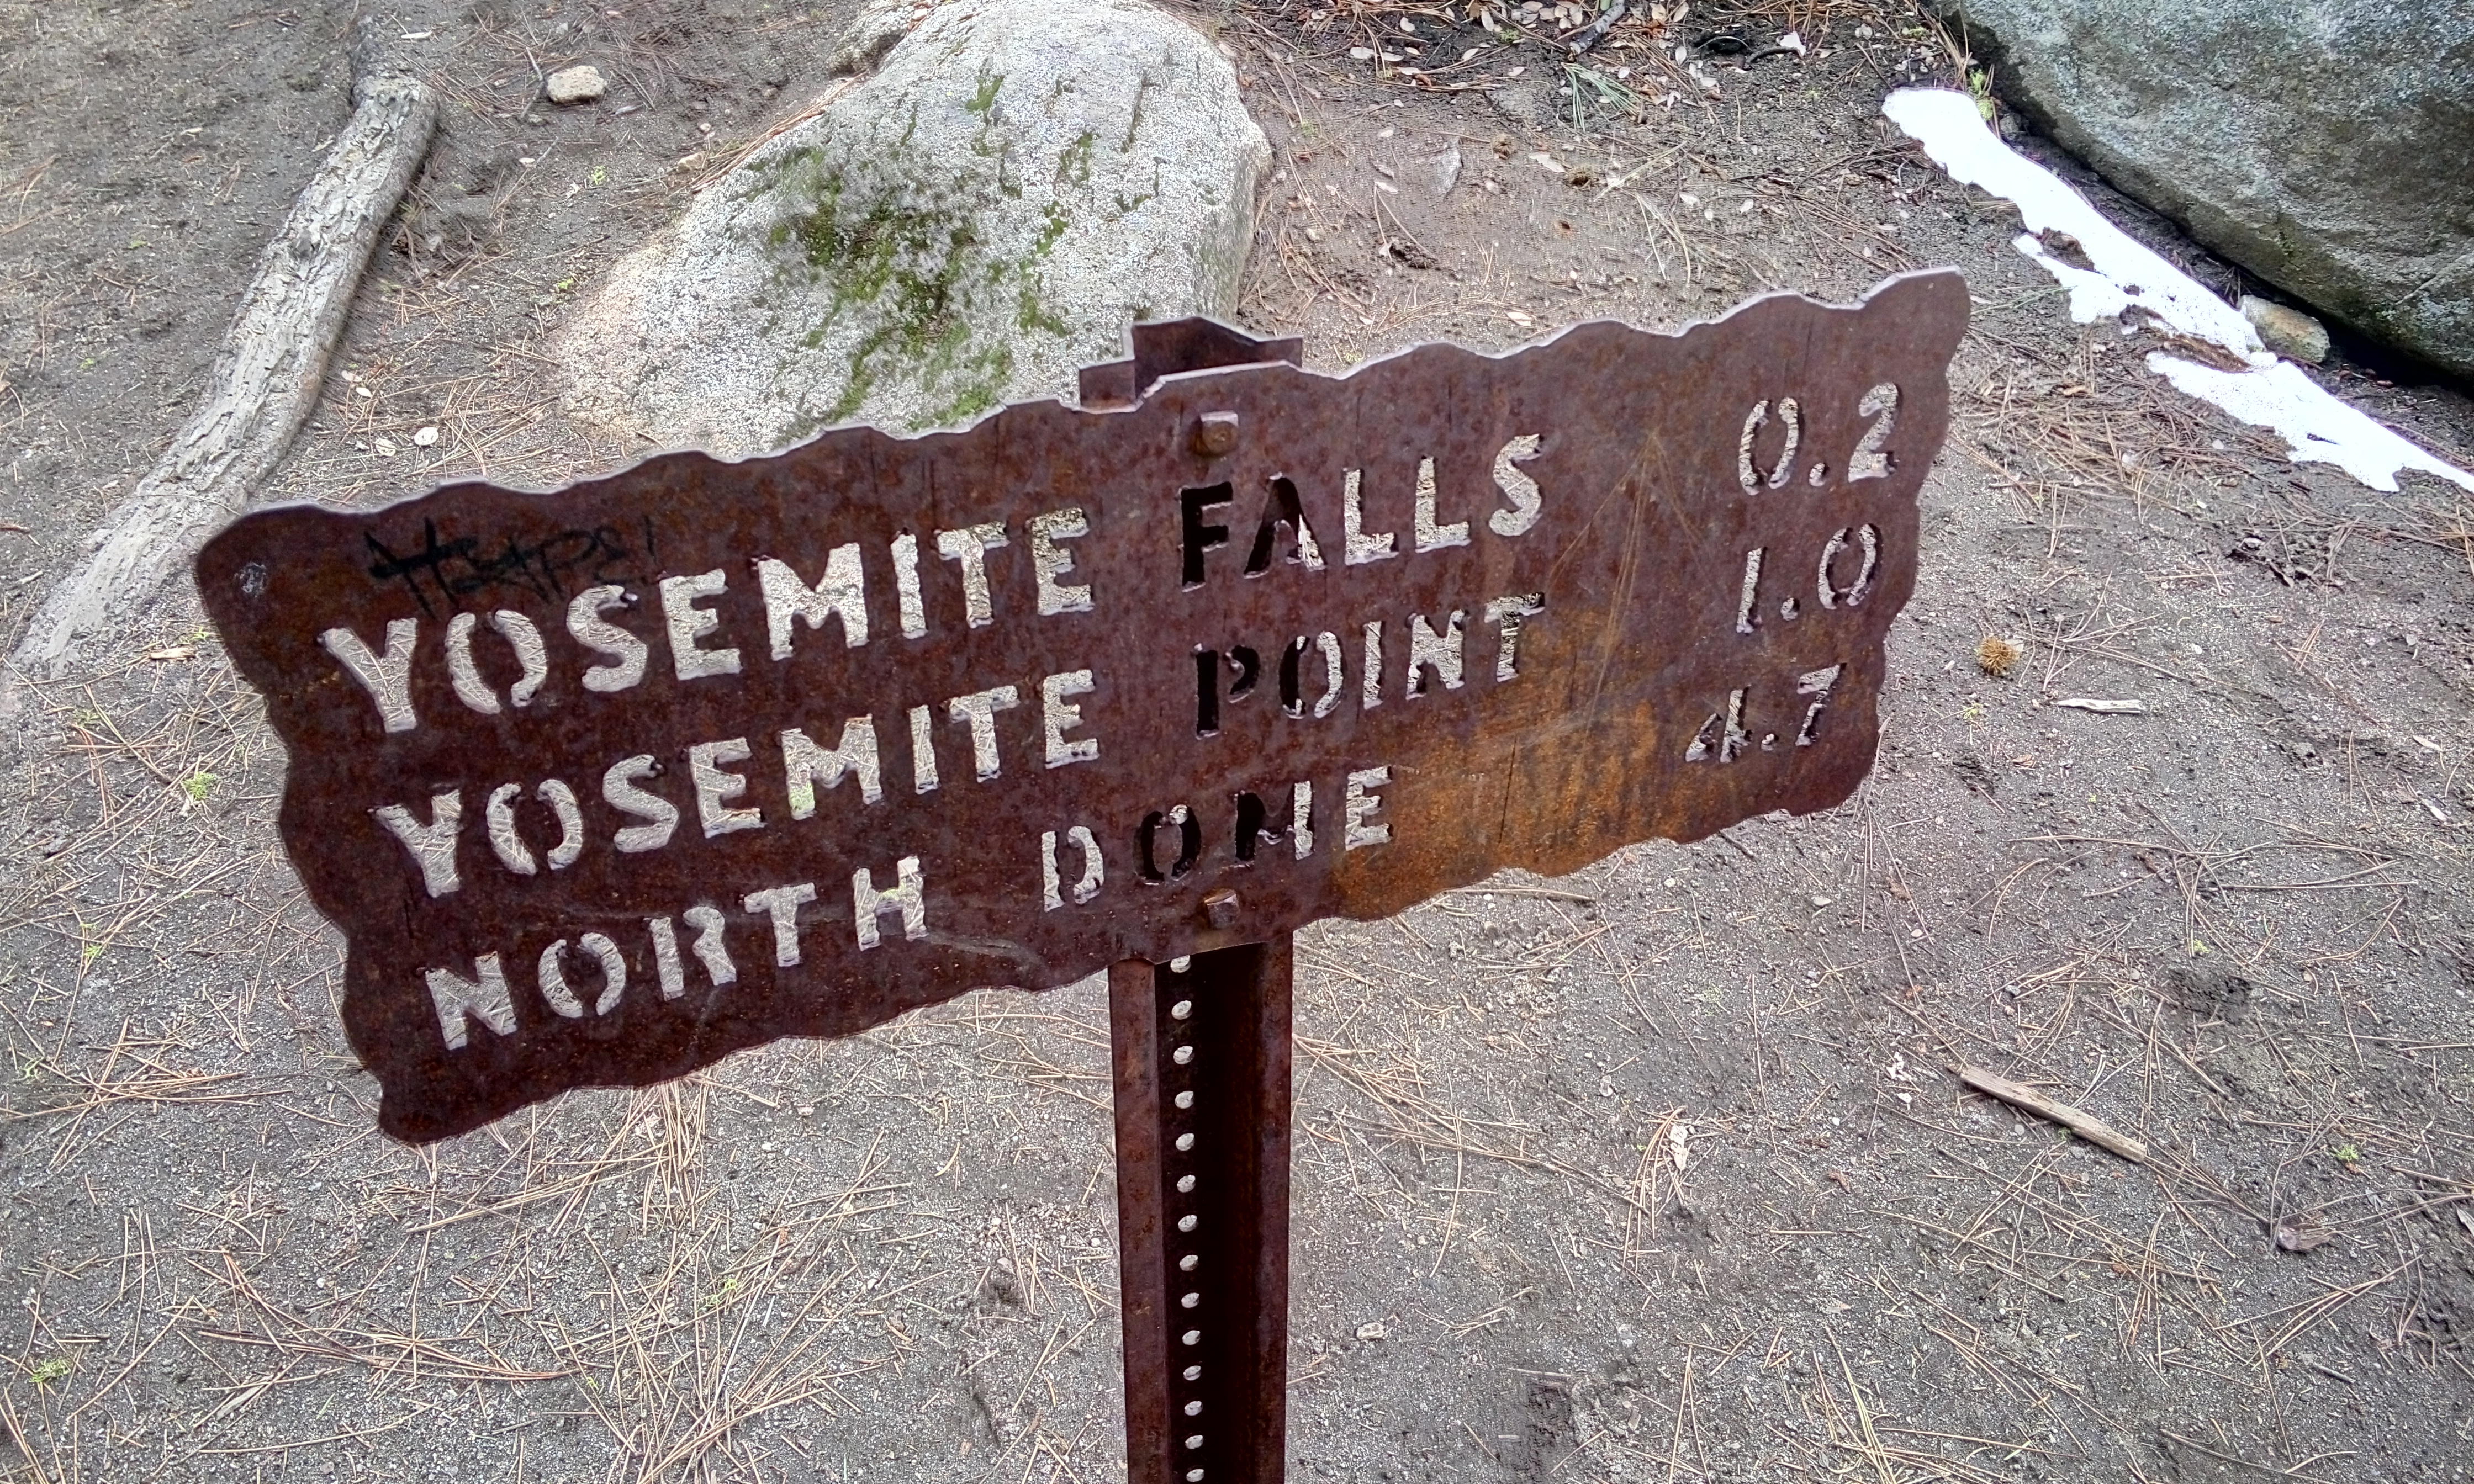
\includegraphics[angle=0,width=\paperwidth,height=.5\paperheight]{24/image20160424_143729995.jpg};%
};
\end{tikzpicture}

Dort gingen wir mal etwas gehobener Essen und siehe da, beim 24~\$ Beef Steak war eine Vorspeise mit dabei und die Crème Brulée stellten sie uns auch nicht in Rechnung.
Insgesamt war das Abendessen nicht wesentlich teurer als sonst, dafür geschmacklich 1a.

\newpage
\thispagestyle{empty}
\begin{tikzpicture}[remember picture, overlay]
\node[inner sep=0pt, yshift=.25\paperheight] at (current page.south) {%
	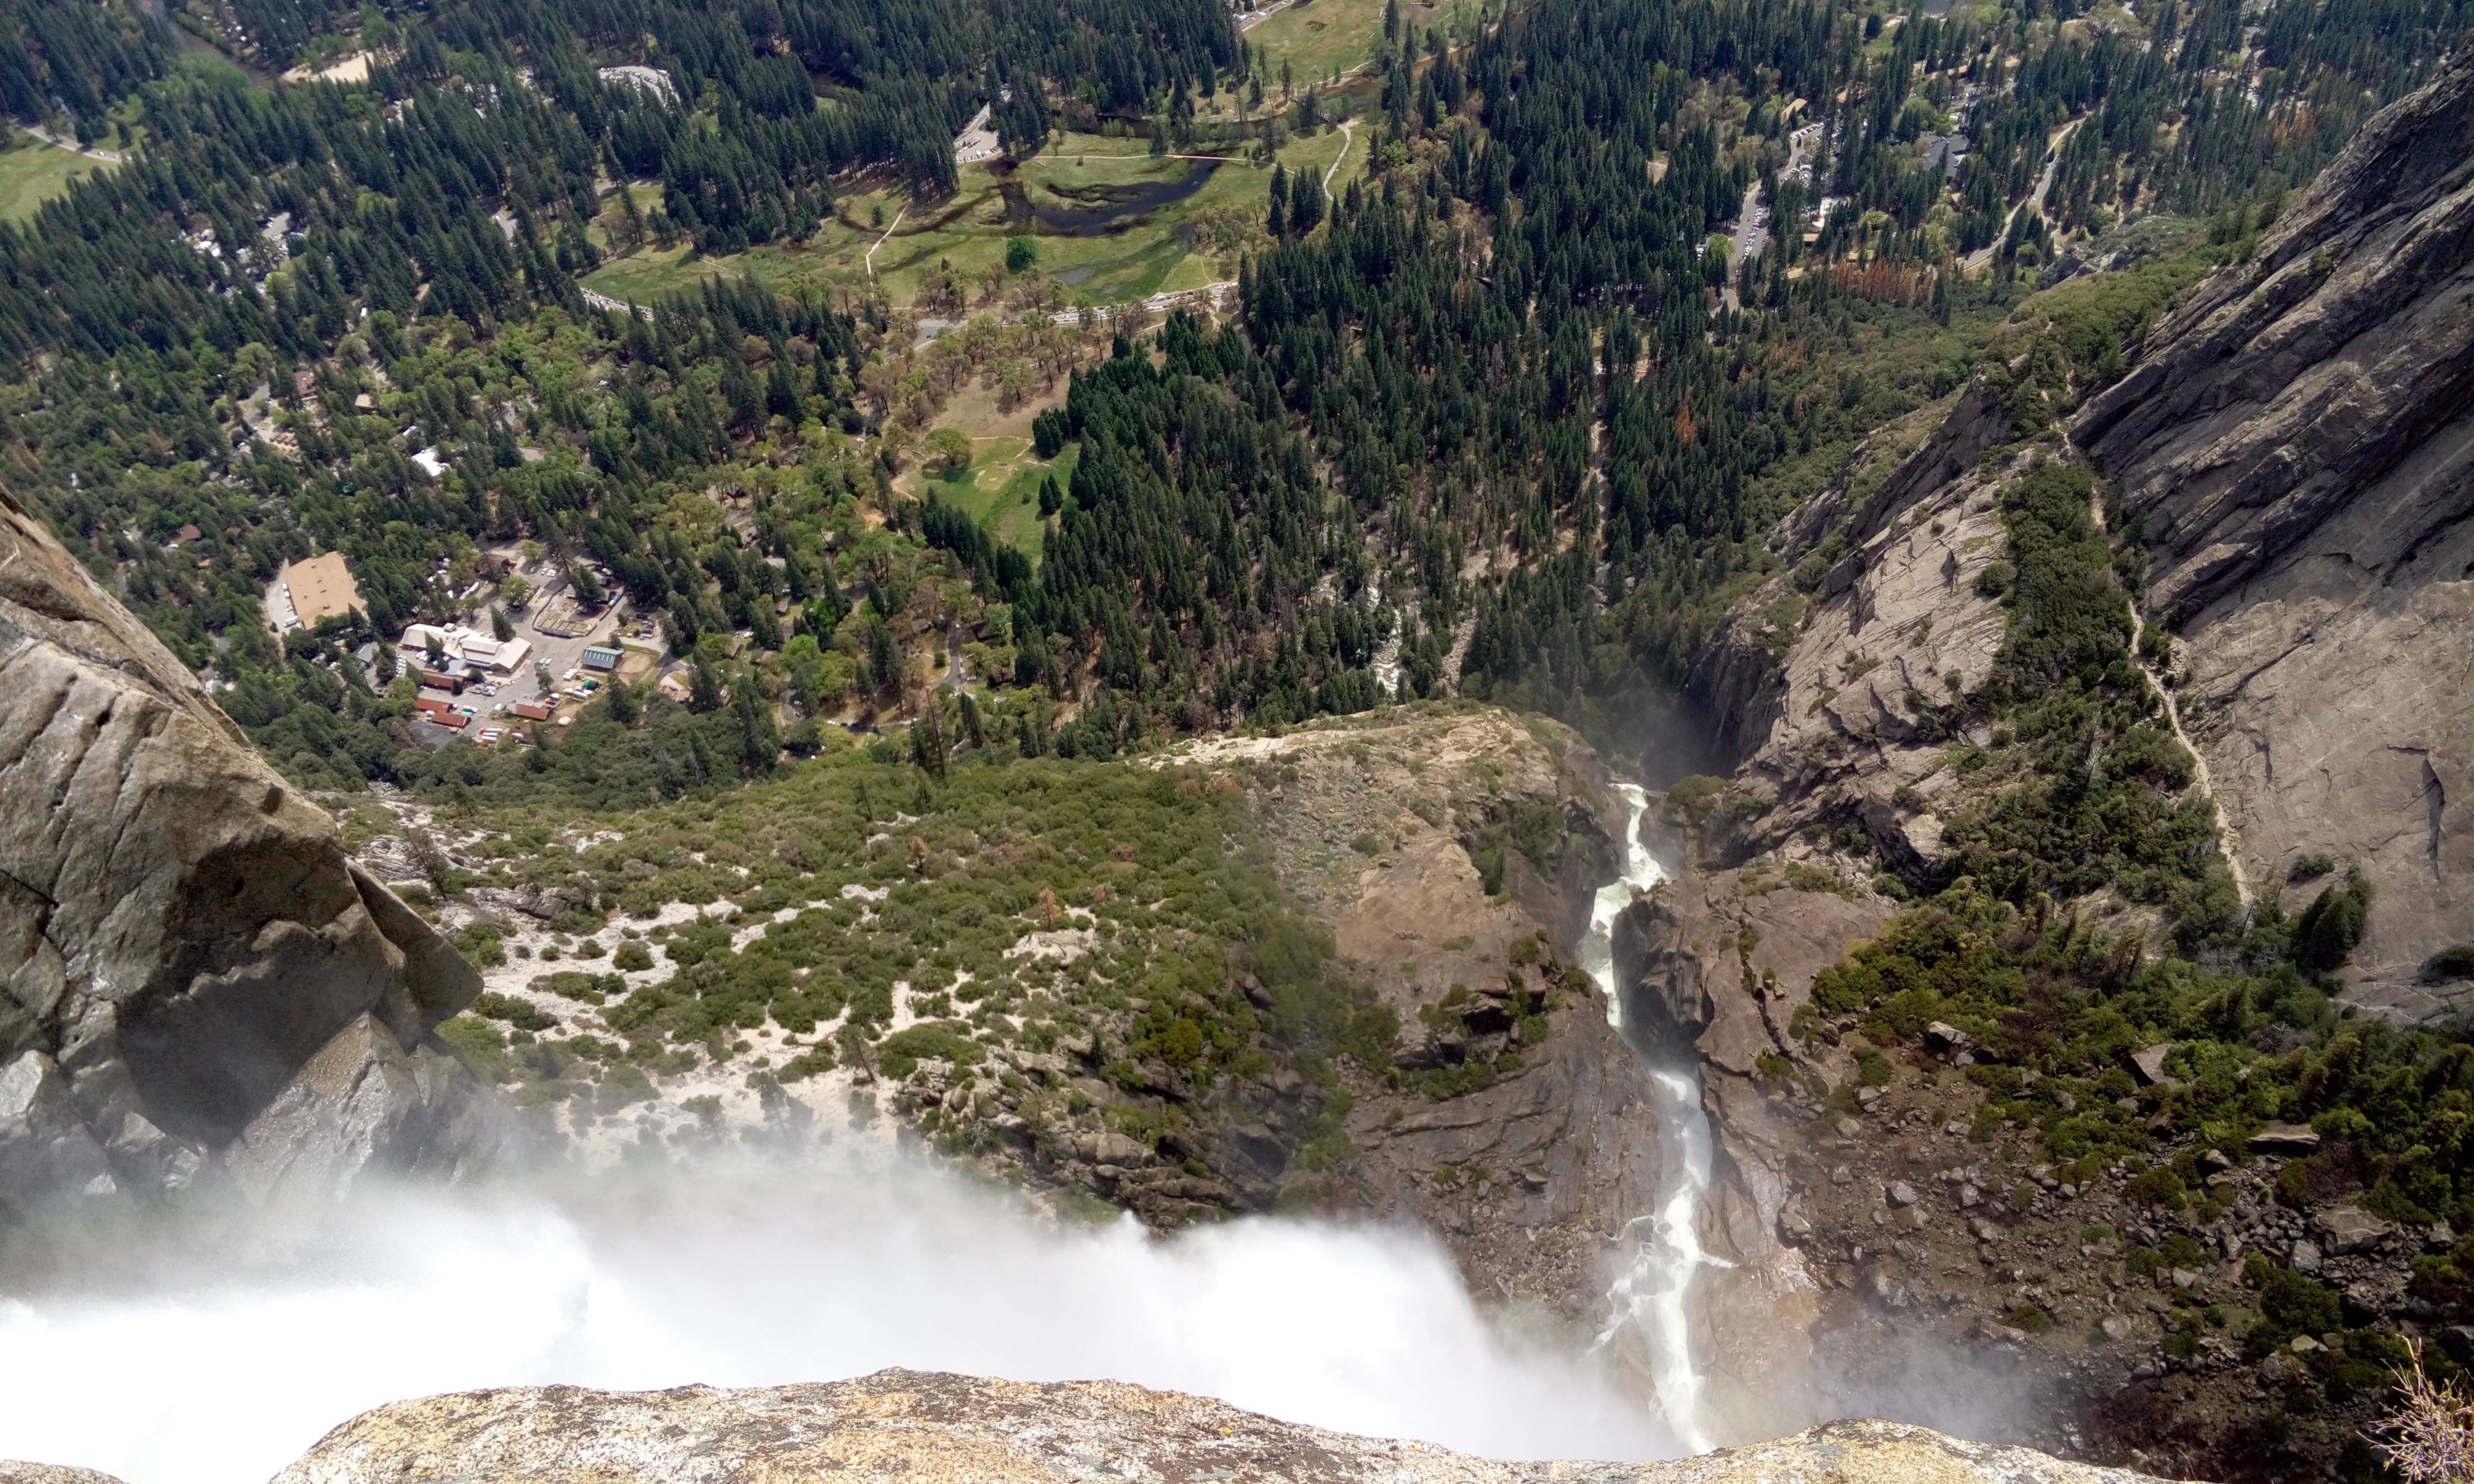
\includegraphics[angle=0,width=\paperwidth,height=.5\paperheight]{24/image20160424_132955369.jpg};%
};
\node[inner sep=0pt, yshift=-.25\paperheight] at (current page.north) {%
	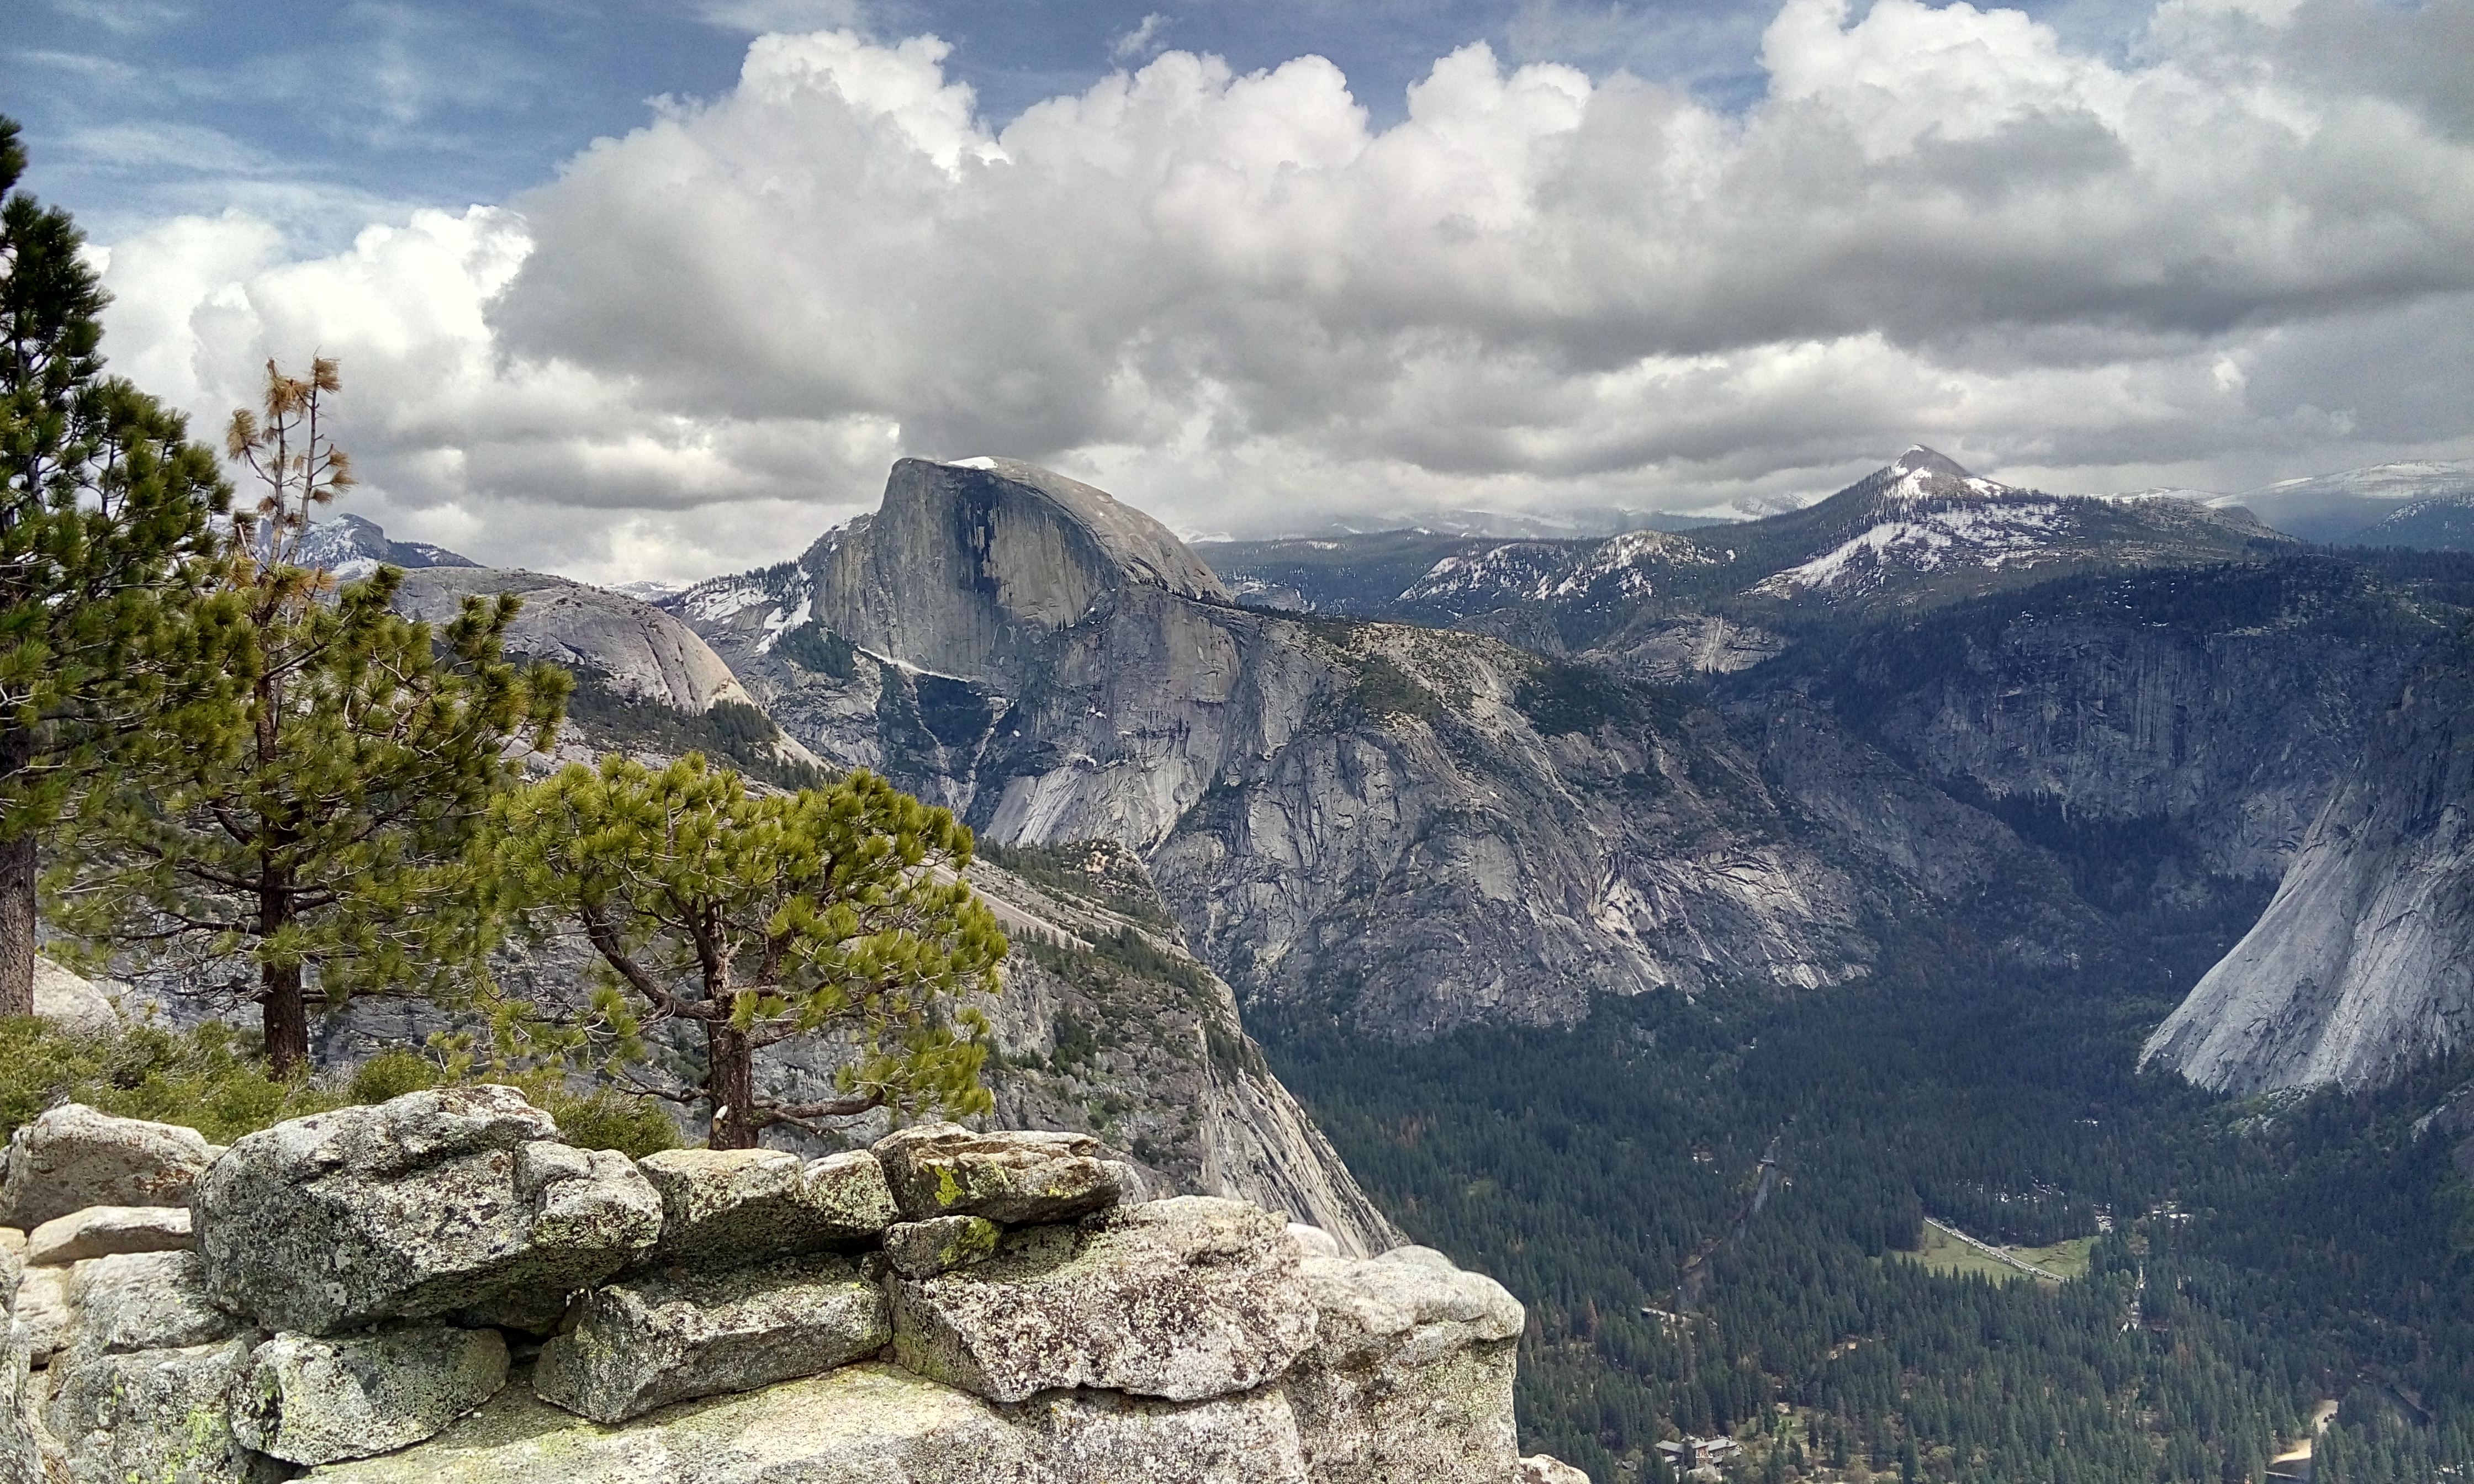
\includegraphics[angle=0,width=\paperwidth,height=.5\paperheight]{24/image20160424_141358732.jpg};%
};
\end{tikzpicture}
\newpage
